\section{Desarrollo completo del producto}

En esta sección podrá encontrar el paso a paso de la solución de \textit{software} D-Minute y la forma que fue abordado en cada \textit{sprint}.

\subsection{Github}

Para el almacenamiento de código fuente se utilizó GitHub, los repositorios que se muestran a continuación tienen la versión instalada en producción:

\begin{table}[!h]
\centering
\resizebox{15cm}{!} {
\begin{tabular}{|l|c|c|l|}
\hline
\multicolumn{1}{|c|}{\textbf{Repositorio}} & \textbf{Tipo} & \textbf{Lenguaje} & \multicolumn{1}{c|}{\textbf{Comentario}} \\ \hline
https://github.com/woliverhl/d-minute-front.git & Front-End & Angular 5 & Versión Front de la aplicación \\ \hline
https://github.com/woliverhl/config-server-dminute.git & Configuración & YML & Contiene los archivos de configuración \\ \hline
https://github.com/woliverhl/d-minute-ms.git & Back-End & Java 1.8 & Versión Back-End de la aplicación \\ \hline
https://github.com/woliverhl/d-minute-zuul.git & \multicolumn{1}{l|}{Zuul} & \multicolumn{1}{l|}{Java 1.8} & Proxy de la aplicación \\ \hline
https://github.com/woliverhl/d-minute-eureka.git & \multicolumn{1}{l|}{Eukera} & \multicolumn{1}{l|}{Java 1.8} & Almacena los microservicios \\ \hline
https://github.com/woliverhl/d-minute-config-server.git & \multicolumn{1}{l|}{Config-Server} & \multicolumn{1}{l|}{Java 1.8} & Entrega la configuración de los servicios \\ \hline
\end{tabular}
}
\end{table}    

\subsection{Dockerhub}

Dado que se utilizó arquitectura digital para el desarrollo de la solución, las imágenes generadas por cada proyecto descrito anteriormente fueron almacenadas en dockerhub, en los siguientes repositorios:


\begin{table}[!h]
\centering
\resizebox{15cm}{!} {
\begin{tabular}{|l|c|l|}
\hline
\multicolumn{1}{|c|}{\textbf{Repositorio}} & \textbf{Tipo} & \multicolumn{1}{c|}{\textbf{Comentario}} \\ \hline
docker pull ohidalgoleal/d-minute-front & Front-End & Contiene la imagen del front-end productivo \\ \hline
docker pull ohidalgoleal/d-minute-ms & Back-End & Contiene la imagen del back-end productivo \\ \hline
docker pull ohidalgoleal/d-minute-zuul & Zuul & Contiene la imagen del proxy productivo \\ \hline
docker pull ohidalgoleal/d-minute-eureka & Eukera & Contiene la imagen de eureka productivo \\ \hline
docker pull ohidalgoleal/d-minute-config-server & Config-Server & Contiene imagen del servidor de configuración \\ \hline
\end{tabular}
}
\end{table} 

\subsection{Detalle de \textit{Sprint}}

\begin{itemize}
	\item \textbf{\textit{Sprint} 1:} Configurar ambientes para desarrollo.

\begin{itemize}
\item \textit{Spring Backlog}

\begin{table}[!h]
\centering
\label{tab:backlog1}
\begin{tabular}{|l|l|r|}
\hline
\multicolumn{1}{|c|}{\textit{\textbf{Feature}}} & \textbf{Epica} & \textbf{Peso} \\ \hline
Configuración ambiente DMinute & Técnica & 3 \\ \hline
Levantar aplicación web en Heroku & Técnica & 3 \\ \hline
Refactorización de código para creación de temas de la reunión & Técnica & 8 \\ \hline
\end{tabular}
\end{table}

\item Desarrollo: Este \textit{sprint} fue completamente técnico, en primera instancia se configuró el ambiente de desarrollo que nos permitió realizar las primeras líneas de código de la aplicación posteriormente se comenzó a realizar pruebas de concepto con el PaaS de Heroku con resultados satisfactorios, desplegando un servicio “demo”. Por último, una historia de usuario consistía en crear el modelo de datos de un acta de reunión que pudiera soportar los elementos de diálogo y sus respectivos temas.

\item \textit{Spring Review}: Como el \textit{sprint} era netamente técnico no hubo resultados que mostrar al PO, sin embargo se presentó los resultado del modelo de datos (ver figura C1) y el PaaS para desplegar los futuros microservicios.

\begin{figure}[!h]
\centering
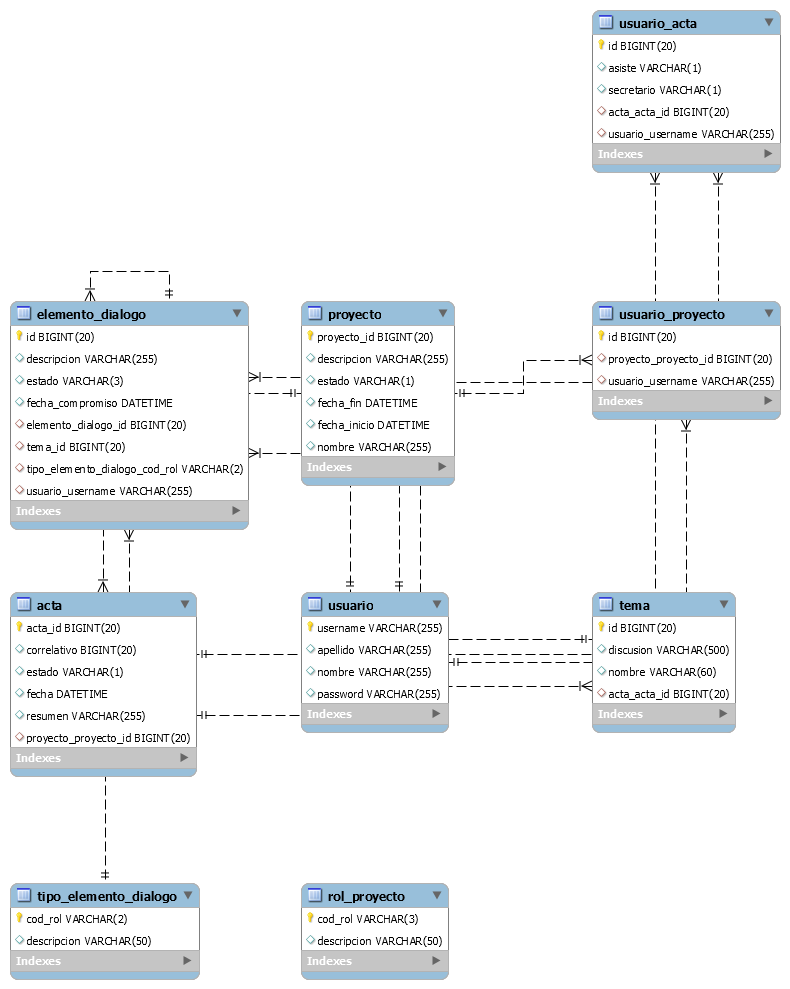
\includegraphics[width=0.7\linewidth]{/modelodminute}
\label{imga-c1}
\caption{Modelo datos crear acta, elaboración propia}
\end{figure}

\end{itemize}


	\item \textbf{\textit{Sprint} 2:} Desarrollar APIs de servicios para la creación de actas y elementos de diálogo.

\begin{itemize}
\item \textit{Spring Backlog}

\begin{table}[!h]
\centering
\label{tab:backlog2}
\begin{tabular}{|l|l|r|}
\hline
\multicolumn{1}{|c|}{\textit{\textbf{Feature}}} & \textbf{Epica} & \textbf{Peso} \\ \hline
Refactorización de código para creación elementos de diálogo & Técnica & 8 \\ \hline
Refactorización de código para creación de minutas & Técnica & 8 \\ \hline
\end{tabular}
\end{table}

\item Desarrollo: Como se indicó en el punto anterior, la aplicación tenía que ser reconstruida, por tanto en este \textit{sprint} se trabajó en migrar el código desarrollado en python a su nueva estructura de java con microservicios. Un trabajo muy complicado que estuvo hasta el último minuto de no ser logrado pues había que estudiar python para ir traspasando las funciones del proyecto al nuevo lenguaje java. Esta tarea se tornó compleja dada la complejidad de manejar ambos lenguajes, pero el trabajo colaborativo permitió crear la sección de minutas y elementos de diálogo como API,s desplegar en heroku para ser utilizadas en los próximos \textit{sprint}. Respecto a la base datos, se estuvo trabajando tanto en la creación de las tablas como en su configuración en la nube con el objetivo de entregar las primeras API`s del servicio.

\item \textit{Spring Review}: Para esta review era importante mostrar software funcionando sin embargo y dado que la parte front-end era muy pesada de construir en términos de puntos. Se presentaron las APIs construidas utilizando postmand\footnote{Definición en: \url{https://www.getpostman.com/}} (ver figura C2).

\begin{figure}[!h]
\centering
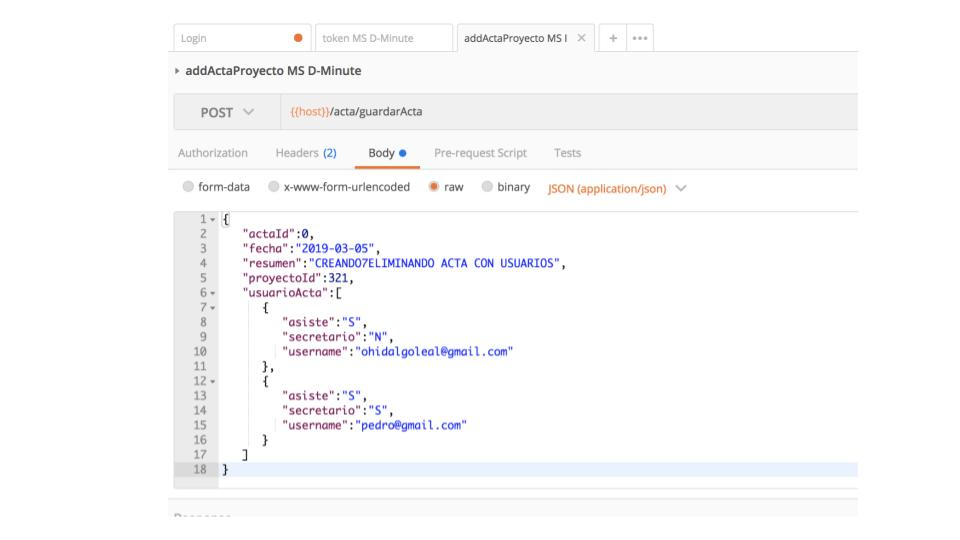
\includegraphics[width=0.8\linewidth]{/postmand}
\label{imga-c2}
\caption{Demostración servicio creación de acta, elaboración propia}
\end{figure}

\end{itemize}


	\item \textbf{\textit{Sprint} 3:} Generar estructura de proyecto \textit{front-end} en angular 5. 

\begin{itemize}
\item \textit{Spring Backlog}

\begin{table}[!h]
\centering
\label{tab:backlog3}
\begin{tabular}{|l|l|r|}
\hline
\multicolumn{1}{|c|}{\textit{\textbf{Feature}}} & \textbf{Epica} & \textbf{Peso} \\ \hline
Implementación nueva estructura UX & Técnica & 8 \\ \hline
Eliminar envio de correo en creación usuario & Técnica & 3 \\ \hline
Cambiar librería de input de textos & Generación Acta & 3 \\ \hline
\textit{Spike} -  Revisar librería Kanban tareas & Seguimiento de tareas & 2 \\ \hline
\end{tabular}
\end{table}

\item Desarrollo: Para el desarrollo de este \textit{sprint} no hubo intenciones de aumentar la velocidad como en el \textit{sprint} anterior debido a que la complejidad de migrar código de un lenguaje a otro es bastante complejo además de que parte del equipo estaría enfocado en investigación (\textit{spike}) con el objetivo de revisar la implementación de un tablero Kanban para el seguimiento de tareas que derivan de los compromisos individuales. La implementación de esta nueva estructura de UX tiene relación a la migración de código python a código angular 5 lo que convella a generar la estructura de carpeta y módulos necesarios para la base de nuestro front-end, uso de nuevas librerías para cuadros de texto y eliminar durante la migración de código el envío de correo en la generación de actas. Lo que corresponde al \textit{spike} se investigó librerías desarrolladas en node, java script y python sin resultados esperados.

\item \textit{Spring Review}: Para el desarrollo de este \textit{sprint} hubo avances significativos de cara al \textit{front-end}. Se presenta su estructura de proyecto en angular 5 y el despliegue del mismo en Heroku. Para el spike si bien se encontró documentación no se pudo seguir investigando pues el equipo se enfocó en terminar el desarrollo de las HDU por tanto no se completaron todos los puntos del \textit{sprint}.

\begin{figure}[!h]
\centering
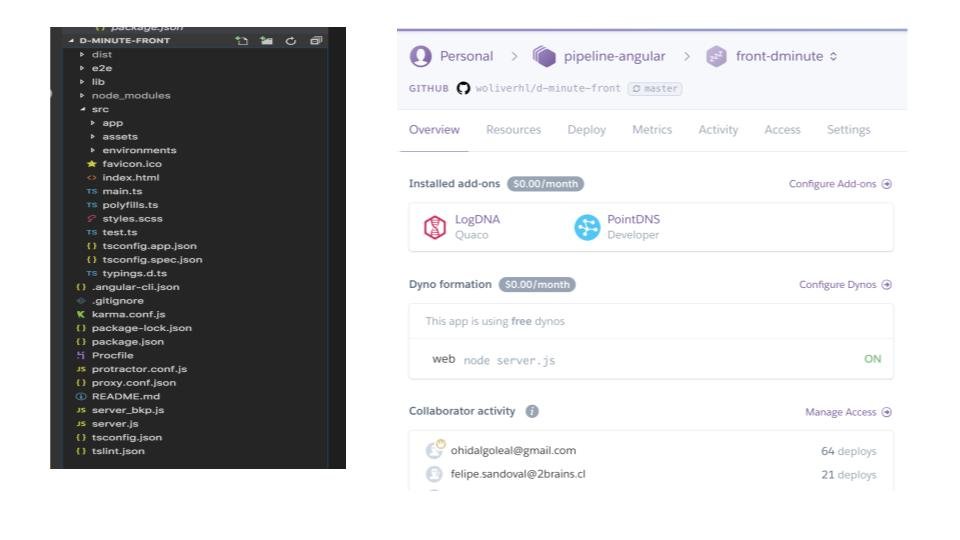
\includegraphics[width=0.8\linewidth]{/demosprint3}
\label{imga-c3}
\caption{Proyecto angular y despliegue en Heroku, elaboración propia}
\end{figure}

\end{itemize}


	\item \textbf{\textit{Sprint} 4:} Migrar por completa aplicación de python a microarquitectura e implementar modelo final de base datos. 

\begin{itemize}
\item \textit{Spring Backlog}

\begin{table}[!h]
\centering
\label{tab:backlog4}
\begin{tabular}{|l|l|r|}
\hline
\multicolumn{1}{|c|}{\textit{\textbf{Feature}}} & \textbf{Epica} & \textbf{Peso} \\ \hline
Reestructurar Menú Creación de Actas & Evolución UX & 5 \\ \hline
Reestructurar Listado de Minutas & Evolución UX & 8 \\ \hline
\end{tabular}
\end{table}

\item Desarrollo: Durante el desarrollo de este \textit{sprint} se abordó la parte front-end de acuerdo a la nueva estructura de UX diseñada previo al \textit{sprint} uno y complementada con el desarrollo de API`s del \textit{sprint} anterior. Dado el nuevo diseño fue necesario generar el modelo final de la base datos que aborda desde el inicio de sesión, el listado de proyectos, las actas de reunión y los elementos del diálogo de cada tema. 

El nuevo diseño de la aplicación llevó a construir la primera parte visual del prototipo, lo anterior generó una tarea bastante complicada que estaba relacionada a la creación de un servidor nginex\footnote{Servidor Nginex: \url{https://es.wikipedia.org/wiki/Nginx}} para que Heroku pudiese desplegar la aplicación en Angular 5 de forma correcta.

\item \textit{Spring Review}: Este es sin duda un \textit{sprint} importante pues se logró visualizar el primer prototipo de la aplicación en base al diseño de UX generado. Se pudo apreciar el modelo de base datos para la creación de actas dialógicas y se logró finalizar los puntos comprometidos de manera exitosa durante el \textit{sprint} (ver figuras: C4, C5 y C6).

\begin{figure}[!h]
\centering
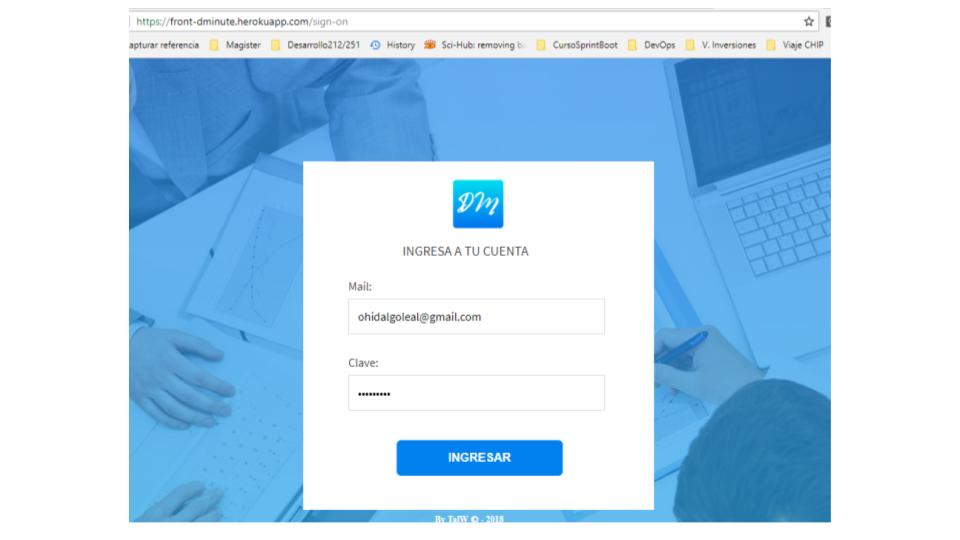
\includegraphics[width=0.8\linewidth]{/demo4-1}
\label{imga-c41}
\caption{Login D-Minute, elaboración propia}
\end{figure}

\begin{figure}[!h]
\centering
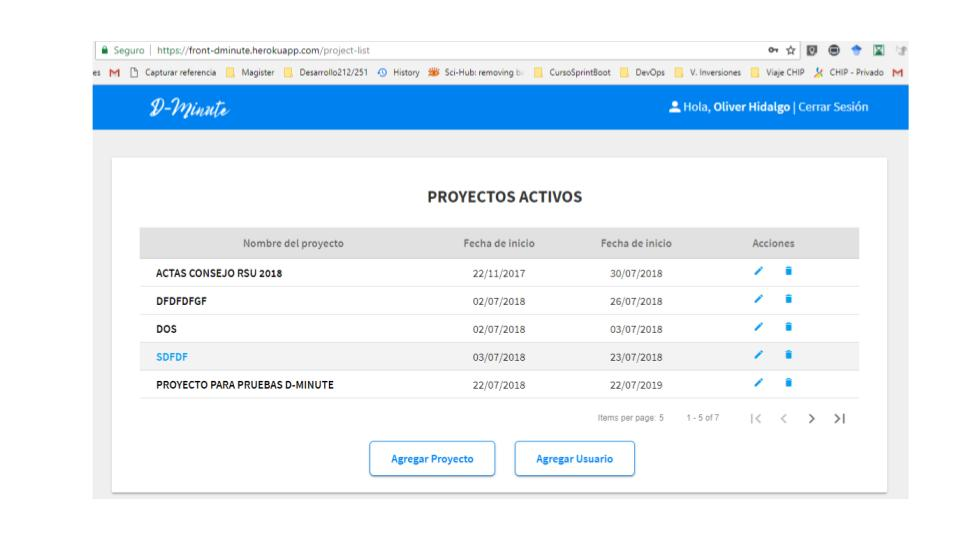
\includegraphics[width=0.8\linewidth]{/demo4-2}
\label{imga-c42}
\caption{Listado proyectos D-Minute, elaboración propia}
\end{figure}

\begin{figure}[!h]
\centering
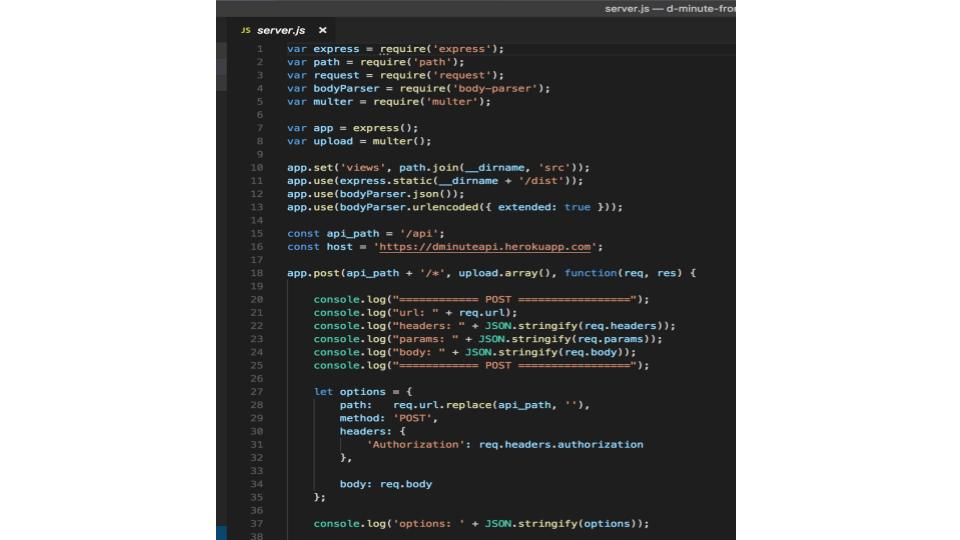
\includegraphics[width=0.8\linewidth]{/demo4-3}
\label{imga-c43}
\caption{Configuración servidor Nginex D-Minute, elaboración propia}
\end{figure}

\end{itemize}


	\item \textbf{\textit{Sprint} 5:} Implementar modelo de micro servicios en \textit{cloud} y generar estilos estándar de la aplicación.

\begin{itemize}
\item \textit{Spring Backlog}

\begin{table}[!h]
\centering
\label{tab:backlog5}
\begin{tabular}{|l|l|r|}
\hline
\multicolumn{1}{|c|}{\textit{\textbf{Feature}}} & \textbf{Epica} & \textbf{Peso} \\ \hline
Normalizar colores aplicación & Evolución UX & 5 \\ \hline
Cargar usuarios nuevos al crear un proyecto & Generación Acta & 5 \\ \hline
Visualizar detalle minuta & Evolución UX & 8 \\ \hline
\end{tabular}
\end{table}

\item Desarrollo: En los \textit{sprint} anteriores hubo un fuerte trabajo por realizar la migración del código desarrollado en python a una nueva arquitectura en java con angular utilizando microsiervos. Este \textit{sprint} está marcado por este último factor, pues era importante comenzar a montar el diseño de arquitectura que hace sostenible la aplicación. Fue necesario comenzar a trabajar en la creación del config server, el registro de eureka y zuul como \textit{proxy server}, todos ellos dentro de un servidor \textit{cloud} Heroku que hace eficiente el desempeño de la aplicación y escalable. 

A los puntos anteriores se suma la creación de minutas, los elementos de diálogo mencionados en el CAPÍTULO 2 sección 2.2 y por último se comenzó a estandarizar los colores de la aplicación reduciendo la deuda técnica adquirida en \textit{sprint} anteriores.

\item \textit{Spring Review}: Durante la \textit{review} de este \textit{sprint} se presentó los componentes desplegados en Heroku que soportan los microservicios que fueron configurados dentro de un pipeline\footnote{Definición y uso de pipeline en: \url{https://jenkins.io/doc/book/pipeline/}} de java y la visualización gráfica de las minutas de un proyecto (ver figuras: C7 y C8).

\begin{figure}[!h]
\centering
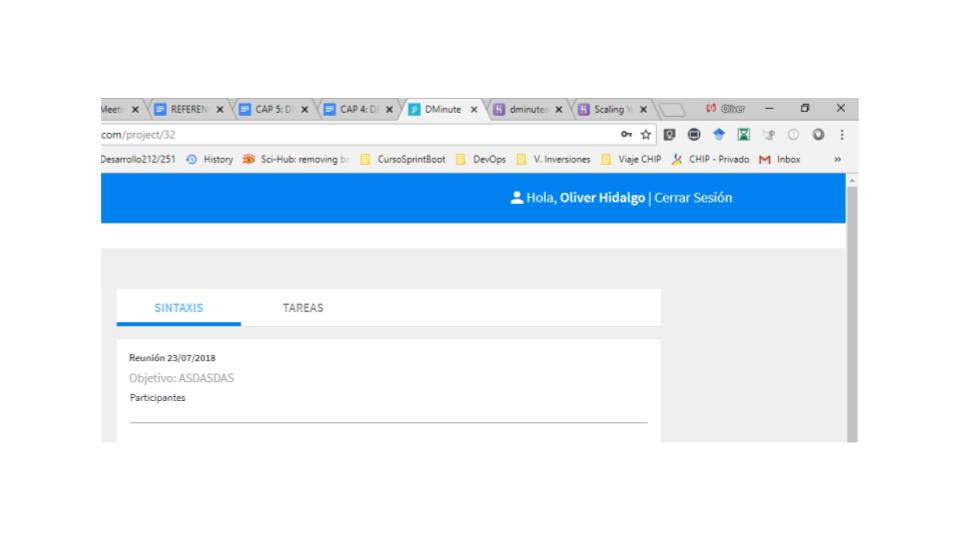
\includegraphics[width=0.8\linewidth]{/demo5-1}
\label{imga-c51}
\caption{Visualizar detalle acta D-Minute, elaboración propia}
\end{figure}

\begin{figure}[!h]
\centering
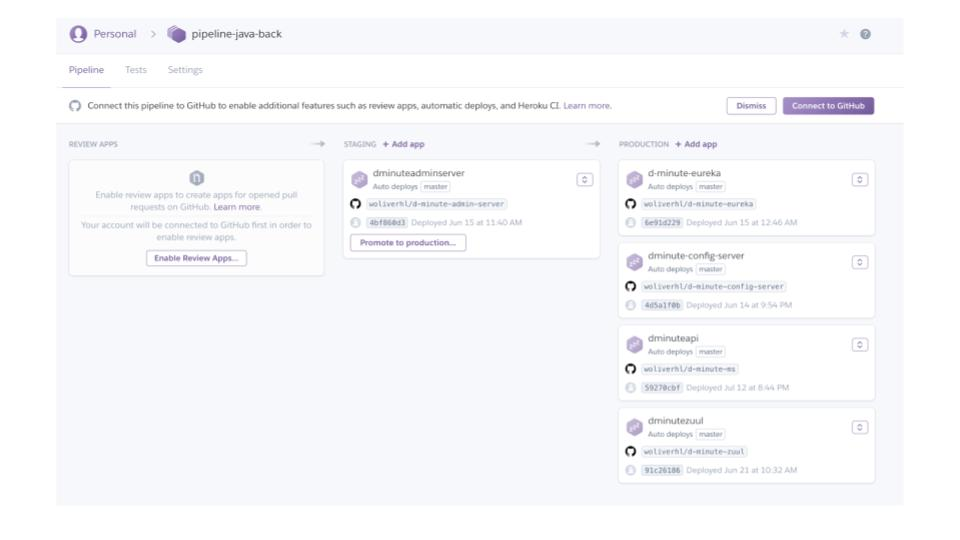
\includegraphics[width=0.8\linewidth]{/demo5-2}
\label{imga-c52}
\caption{Pipeline arquitectura de microservicios D-Minute, elaboración propia}
\end{figure}

\end{itemize}


	\item \textbf{\textit{Sprint} 6:} Mejorar aspectos visuales de la aplicación arrastrados de la migración. 
	
\begin{itemize}
\item \textit{Spring Backlog}

\begin{table}[!h]
\centering
\label{tab:backlog6}
\begin{tabular}{|l|l|r|}
\hline
\multicolumn{1}{|c|}{\textit{\textbf{Feature}}} & \textbf{Epica} & \textbf{Peso} \\ \hline
Texto al agregar elementos de diálogo & Generación Acta & 1 \\ \hline
Eliminación Menú & Evolución UX & 1 \\ \hline
BUG: editar un elemento de diálogo & Generación Acta & 3 \\ \hline
Quitar opción colapsable & Evolución UX & 5 \\ \hline
Nombre en barra superior & Evolución UX & 2 \\ \hline
Calendario en español & Generación Acta & 3 \\ \hline
\end{tabular}
\end{table}

\item Desarrollo: El desarrollo del \textit{sprint} 6 está marcado por mejorar aspectos visuales de la aplicación pues producto de la migración a java y angular algunas características de la aplicación se tomaron de python sin ser cuestionadas. Si bien el producto pretende ser un mínimo viable, se testeó la aplicación con algunos usuarios finales durante el \textit{sprint} 5 lo que permitió incorporar en esta\textit{sprint backlog} historias que permitan mejorar la experiencia de usuario también durante el testeo se detectaron \textit{BUG} que fueron abordados en el \textit{sprint}.

\item \textit{Spring Review}: Como se indicó en el desarrollo, las mejoras del producto fue el punto a revisar durante el \textit{sprint} y los BUG identificados por los usuarios finales (ver figura C9).

\begin{figure}[!h]
\centering
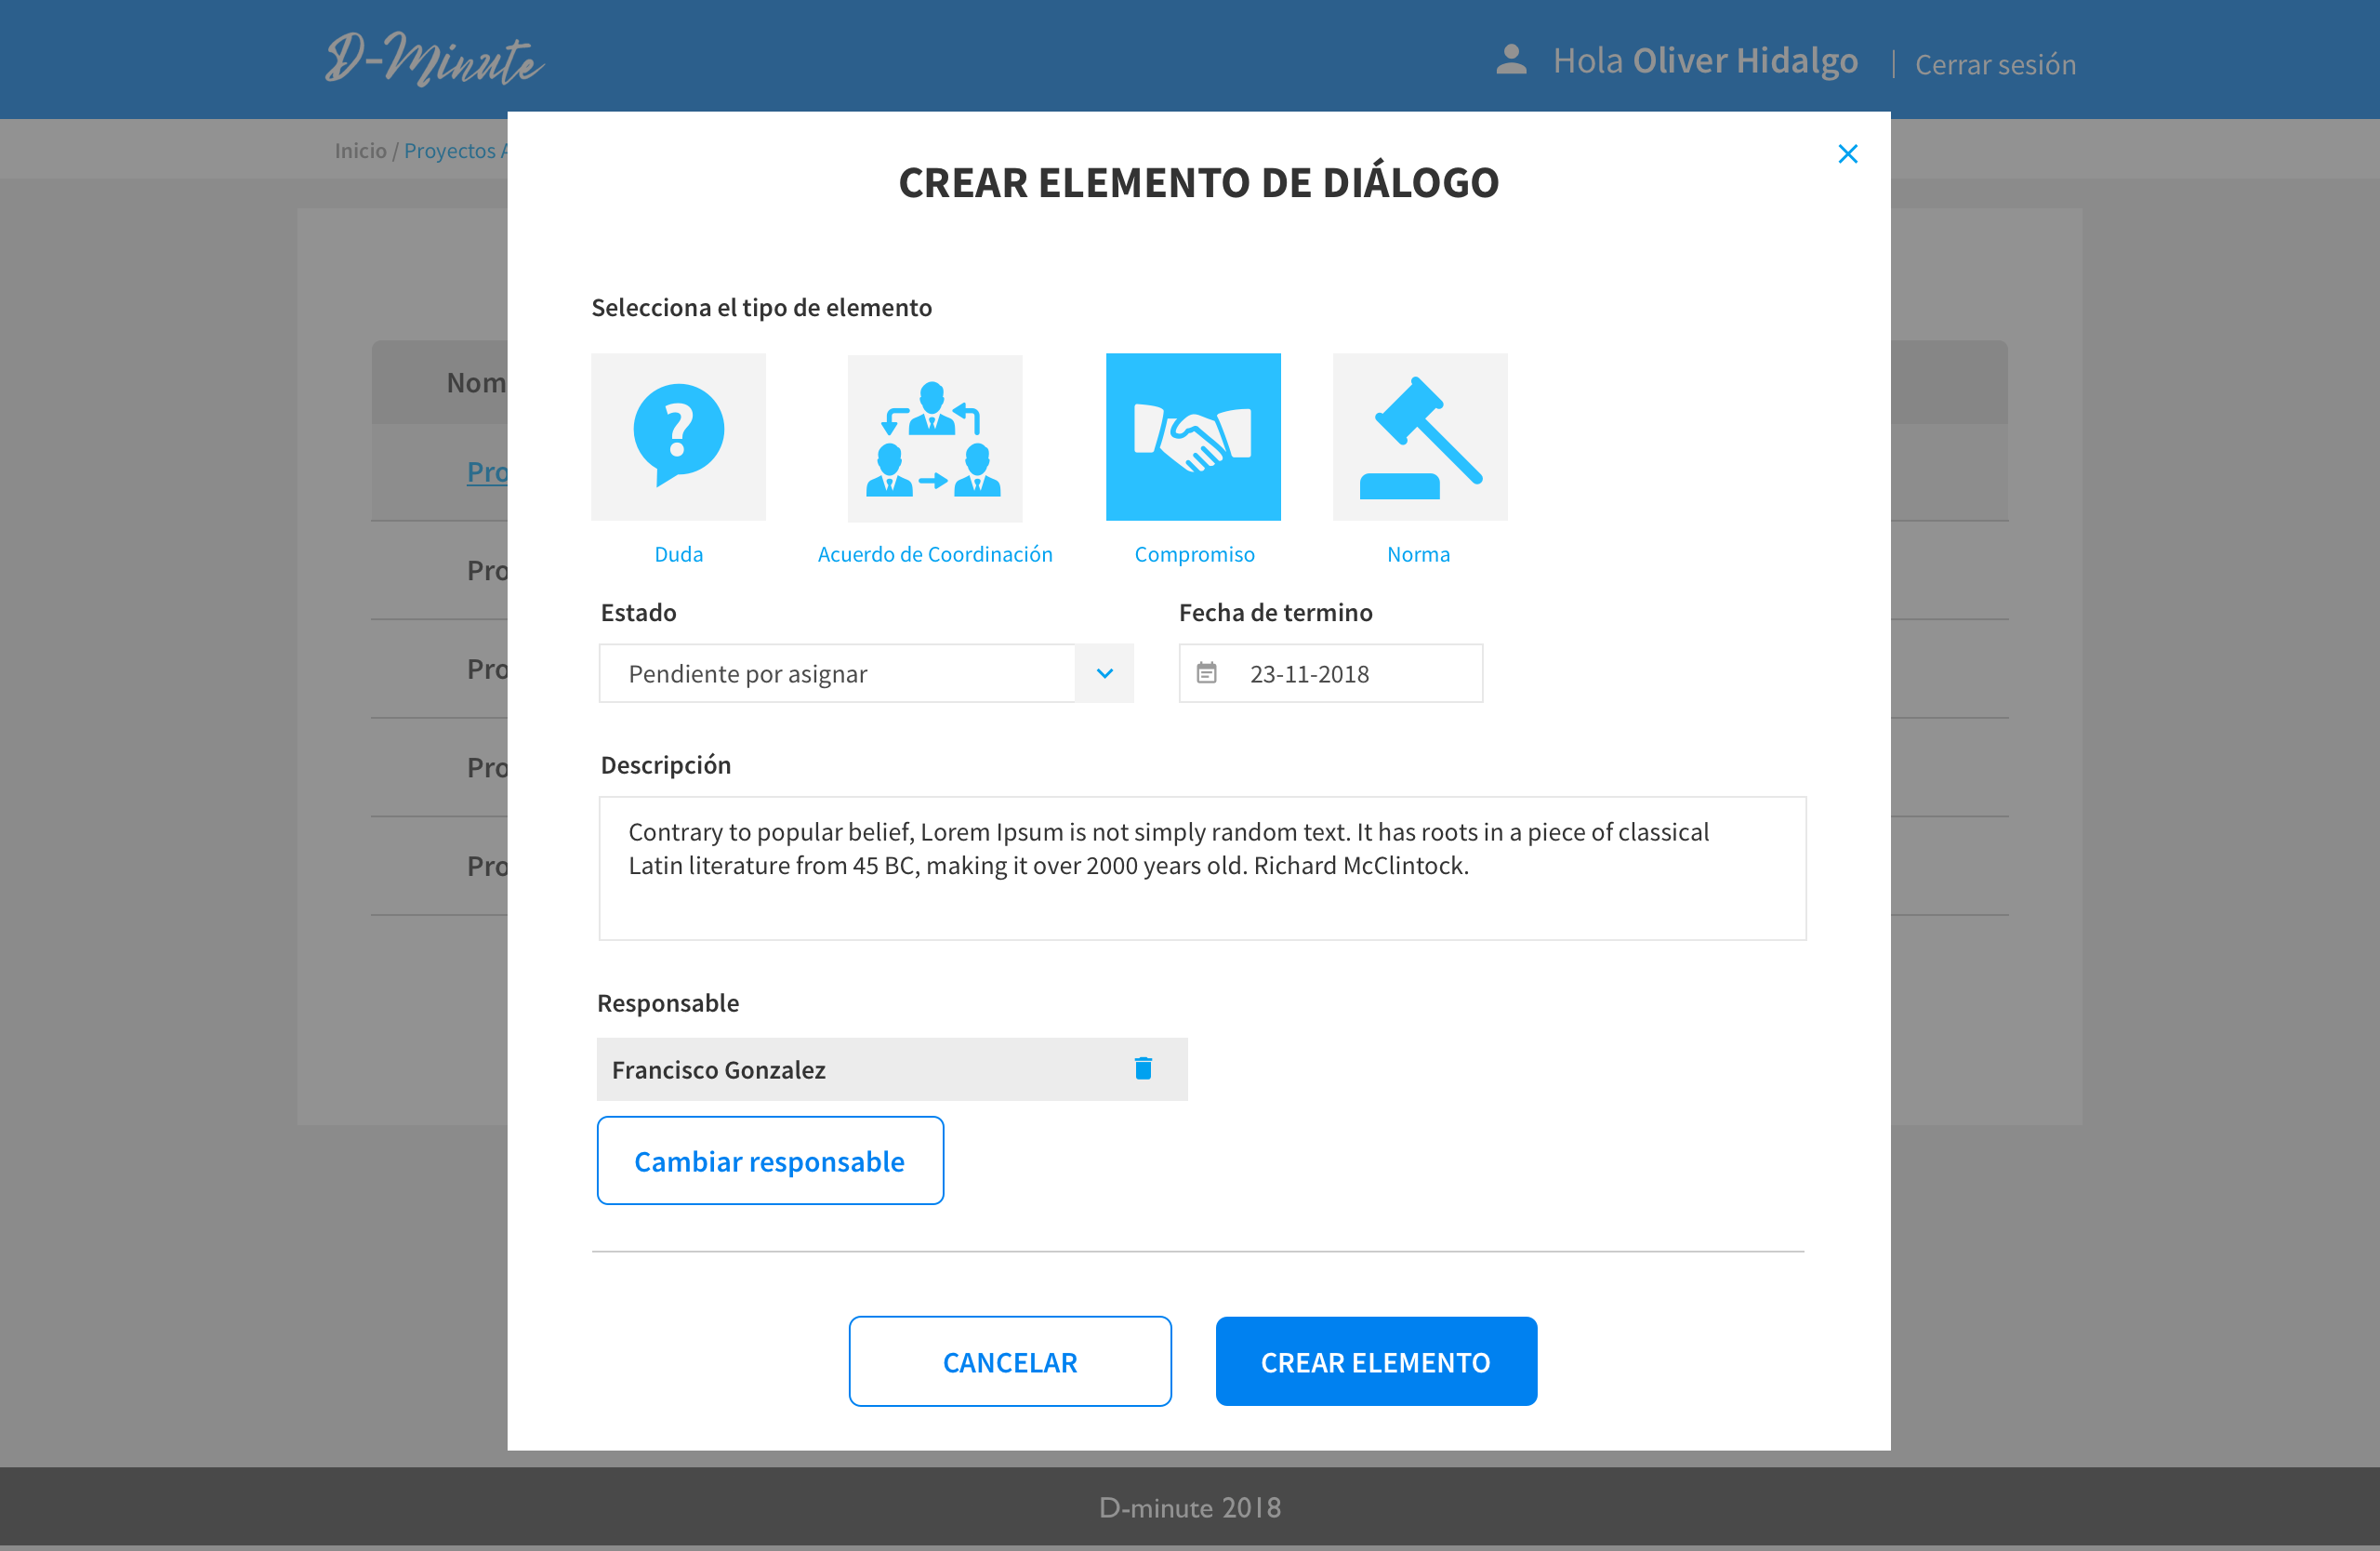
\includegraphics[width=0.8\linewidth]{/demo6}
\label{imga-c6}
\caption{Mejoras al editar elementos de diálogo D-Minute, elaboración propia}
\end{figure}

\end{itemize}	

	\item \textbf{\textit{Sprint} 7:} Implementar nuevo diseño UX y corrección de \textit{bugs} críticos. 

\begin{itemize}
\item \textit{Spring Backlog}

\begin{table}[!h]
\centering
\label{tab:backlog7}
\begin{tabular}{|l|l|r|}
\hline
\multicolumn{1}{|c|}{\textit{\textbf{Feature}}} & \textbf{Epica} & \textbf{Peso} \\ \hline
BUG: seleccionar asistentes de una reunión & Generación Acta & 5 \\ \hline
BUG: al editar y crear un acta & Generación Acta & 5 \\ \hline
Mejora estilo + iconos & Evolución UX & 8 \\ \hline
BUG: Se duplica acta al editar & Generación Acta & 5 \\ \hline
\end{tabular}
\end{table}


\item Desarrollo: Durante el \textit{sprint} 5 y 6 se comenzó el testeo de la aplicación con usuarios finales a fin de identificar puntos de mejora que no se detectaron durante el QA de la aplicación. Resultado de este trabajo fueron \textit{BUGs} importantes que afectaron la funcionalidad del producto y debido a que eran críticos se priorizo la corrección de estos por sobre nuevas funcionalidades, sin embargo debido al mismo testeo de usuarios se incorporó la nueva línea UX en la aplicación pues era la apuesta principal que se apuntaba como equipo, un hito importante considerando que hubo un sobre esfuerzo en términos de\textit{velocity}. 

\item \textit{Spring Review}: El resultado de este \textit{sprint} es sin lugar a dudas uno de los más importantes pues se logró implementar la nueva línea de UX que fue testeada con los usuarios finales. Se marca un cambio en la forma de visualizar las minutas y se incorporan los nuevos iconos de los elementos de diálogo sin dejar de lado los bugs detectados en etapas tempranas (ver figura C10).

\begin{figure}[!h]
\centering
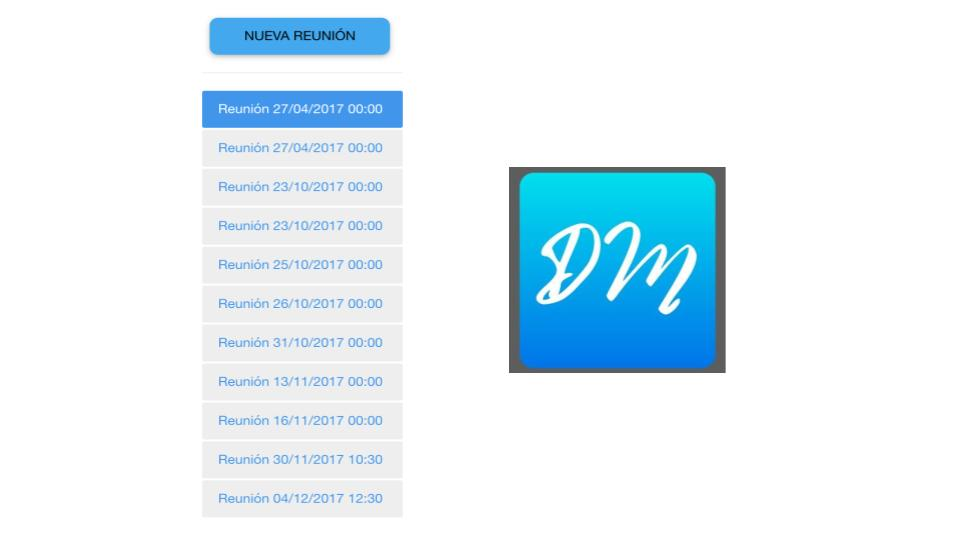
\includegraphics[width=0.8\linewidth]{/demo7}
\label{imga-c7}
\caption{Nuevo logo D-Minute y lista de reuniones, elaboración propia}
\end{figure}

\end{itemize}	


	\item \textbf{\textit{Sprint} 8:} Reducir deuda técnica de \textit{front-end} y \textit{back-end}. 

\begin{itemize}
\item \textit{Spring Backlog}

\begin{table}[!h]
\centering
\label{tab:backlog8}
\begin{tabular}{|l|l|r|}
\hline
\multicolumn{1}{|c|}{\textit{\textbf{Feature}}} & \textbf{Epica} & \textbf{Peso} \\ \hline
Seleccionar Icono al agregar elemento de diálogo & Trazabilidad Elementos & 8 \\ \hline
BUG: Se corta pantalla al agregar elemento de diálogo & Evolución UX & 3 \\ \hline
Quitar espaciado Panel de Proyecto & Evolución UX & 2 \\ \hline
Número reunión & Generación Acta & 5 \\ \hline
\end{tabular}
\end{table}



\item Desarrollo: Nuestro último \textit{sprint} está marcado por mejoras en la aplicación y deuda técnica de backend que eran necesarias para mejorar performance del software, de igual forma se trabajó en aspecto de experiencia de usuario pues una de las características de la aplicación es el concepto usable para ello las HDU indicadas abordan este concepto. Los bug detectados fueron desarrollados por el equipo pero no tenían una alta complejidad como los indicados en el \textit{sprint} anterior.

Lo anterior, permitió al equipo volver a su velocidad de 16 puntos por sobre el esfuerzo extra realizado el \textit{sprint} anterior que el objetivo era concluir la nueva línea de UX.

\item \textit{Spring Review}: La \textit{review} de este \textit{sprint} se enmarca dentro de las mejoras de la aplicación por tanto se presenta al PO los bugs detectados haciendo hincapié en los aspectos técnicos que mejoran la performance de la aplicación.

\end{itemize}

\end{itemize}

